\documentclass{article}
\usepackage{graphicx,float}
\usepackage{amsmath,latexsym,amsfonts,amssymb,amsthm}

\usepackage[utf8]{inputenc}
\usepackage[english]{babel}
\usepackage[letterpaper,top=2cm,bottom=2cm,left=3cm,right=3cm,marginparwidth=1.75cm]{geometry}
\renewcommand{\baselinestretch}{1.667}


\title{Compute Intelligence PS s7 Lab 3 }
\author{Joris Plaščinskas}
\date{\today}


\begin{document}


\maketitle
\section*{Introduction}
The goal of this laboratory work is to classify iris dataset using WEKA software. My student number is 2016020, which means that my variant is: "0. sepal length, sepal width, petal length". Iris dataset will be split into train and test sets at the start (80\% \& 20\%). In figure-\ref{fig:visualize} below you can see how the data is distributed (blue - iris setosa, red - iris versicolor, light blue - iris virginica).
\begin{figure}[H]
    \centering
    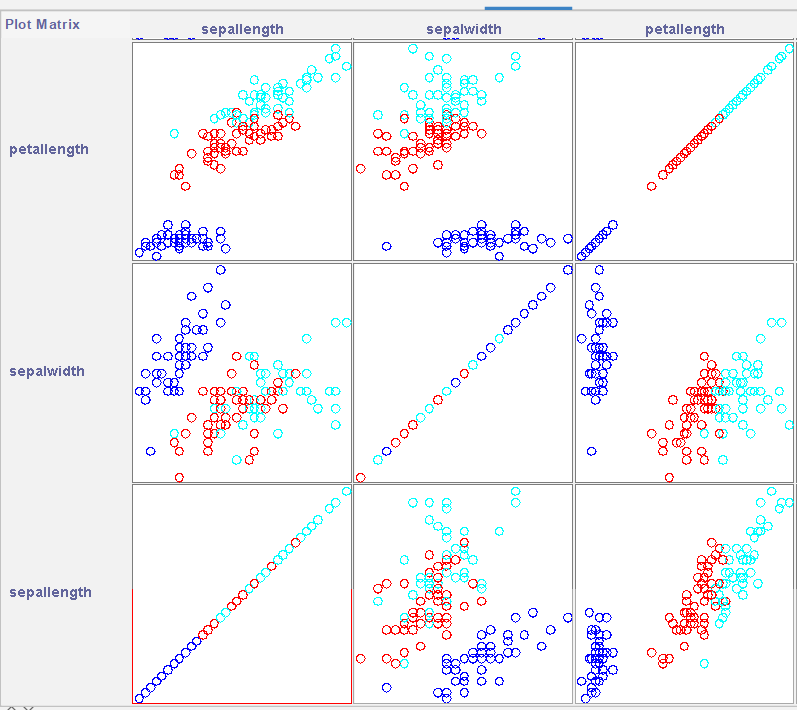
\includegraphics[width=0.5\textwidth]{visualize.png}
    \caption{Iris Data Visualized}
    \label{fig:visualize}
\end{figure}


\section*{Schemes}
\subsection*{Scheme 1}
In figure-\ref{fig:scheme-1} you can see the first scheme. This scheme takes the initial data, pre-processes it, trains a multilayer perceptron and evaluates it's performance. The learning rate and momentum were set to $0.2$, $0.0002$ and hidden layers were: 2,1. I tried changing the parameters, but the accuracy would always end up the same unless I set the learning rate to some extreme value. The performance of the model can be seen below in figure-\ref{fig:confusion}. In figure-\ref{fig:normal} you can see the metrics when normal parameters were used and in figure-\ref{fig:extreme} you can see the results when a very low learning rate was used.
\begin{figure}[H]
    \centering
    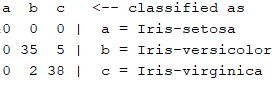
\includegraphics[width=0.3\textwidth]{confusion.png}
    \caption{Confusion Matrix}
    \label{fig:confusion}
\end{figure}
\begin{figure}[H]
    \centering
    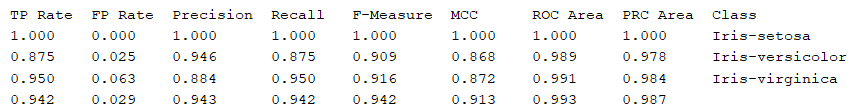
\includegraphics[width=0.8\textwidth]{normal-results.png}
    \caption{Metrics}
    \label{fig:normal}
\end{figure}
\begin{figure}[H]
    \centering
    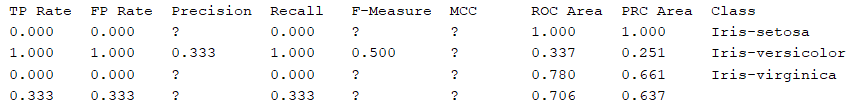
\includegraphics[width=0.8\textwidth]{extreme-results.png}
    \caption{Extreme LR Metrics}
    \label{fig:extreme}
\end{figure}
\begin{figure}[H]
    \centering
    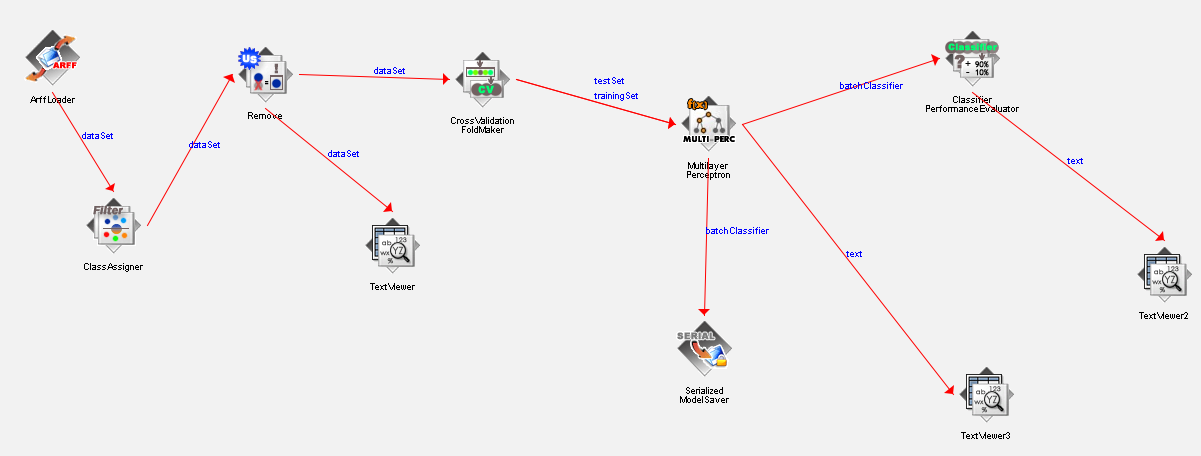
\includegraphics[width=1\textwidth]{config-1.png}
    \caption{Scheme 1}
    \label{fig:scheme-1}
\end{figure}


\subsection*{Scheme 2}
Scheme 2 can be seen in figure-\ref{fig:scheme-2} below. This scheme now adds a prediction appender, that outputs the whole dataset with model predictions attached. Model predictions can be seen in figure-\ref{fig:predictions}. The model performs flawlessly on test data as seen in figure-\ref{fig:metrics-2}
\begin{figure}[H]
    \centering
    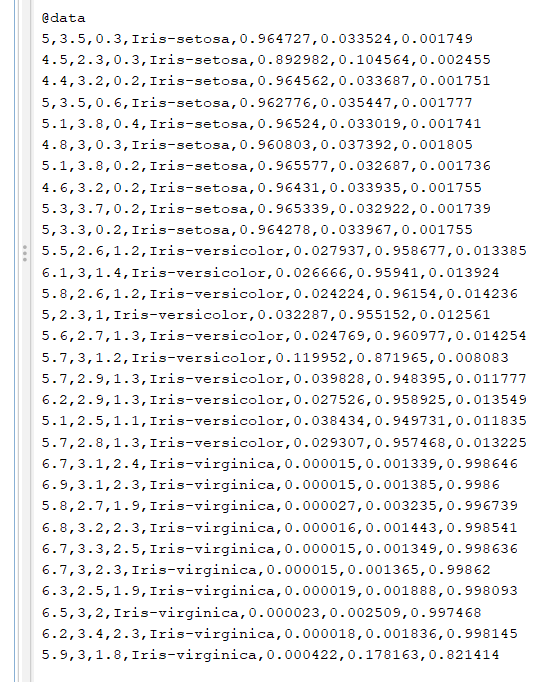
\includegraphics[width=0.5\textwidth]{predictions.png}
    \caption{Predictions}
    \label{fig:predictions}
\end{figure}
\begin{figure}[H]
    \centering
    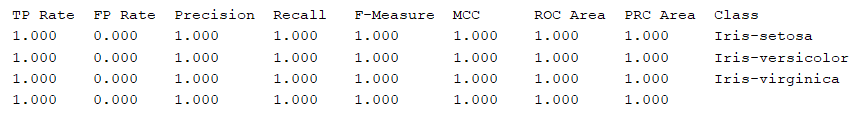
\includegraphics[width=0.8\textwidth]{metrics-2.png}
    \caption{Metrics}
    \label{fig:metrics-2}
\end{figure}
\begin{figure}[H]
    \centering
    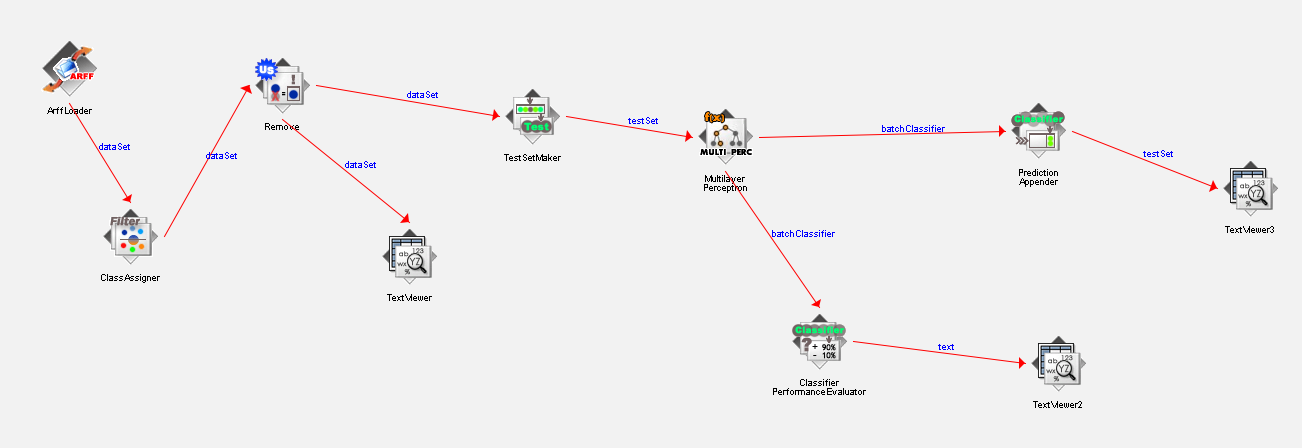
\includegraphics[width=1\textwidth]{config-2.png}
    \caption{Scheme 2}
    \label{fig:scheme-2}
\end{figure}


\subsection*{Scheme 3}
Scheme 3 can be seen in figure-\ref{fig:scheme-3} below. This scheme implements two datasets: train and test. It also outputs model parameters, which will be used later to implement the model in python code.
\begin{figure}[H]
    \centering
    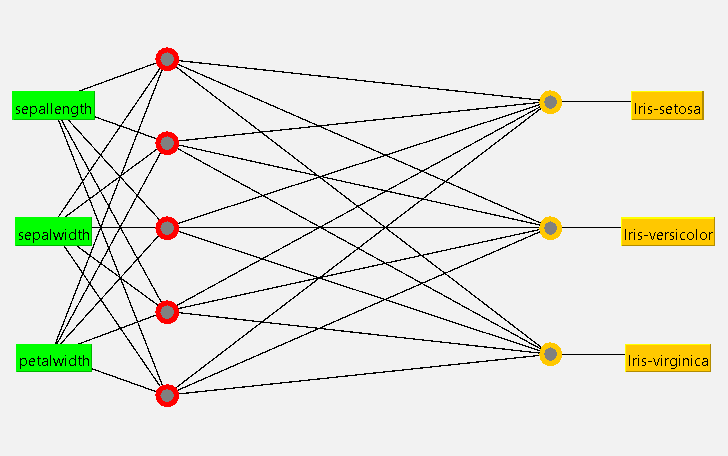
\includegraphics[width=1\textwidth]{model.png}
    \caption{Model}
    \label{fig:model}
\end{figure}
\begin{figure}[H]
    \centering
    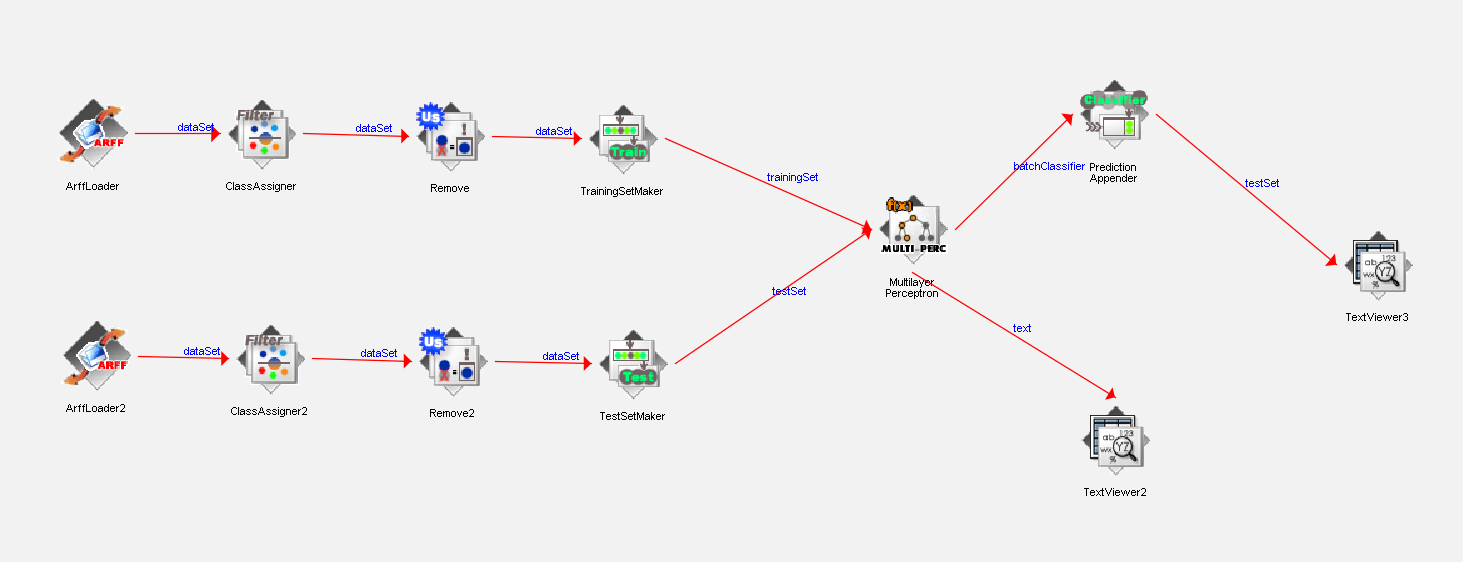
\includegraphics[width=1\textwidth]{config-3.png}
    \caption{Scheme 3}
    \label{fig:scheme-3}
\end{figure}


\section*{Excel - Or Python Code In My Case}
I chose to implement the model in python instaed of Excel. I copy pasted model weights and biases directly into numpy matrices. I implemented sigmoid and softmax functions, then using these functions and matrix multiplication I calculated the predictions, which I then processed into labels, the whole code can be seen below. Model parameters can be seen in figure-\ref{fig:scheme-3}.
\begin{figure}[H]
    \centering
    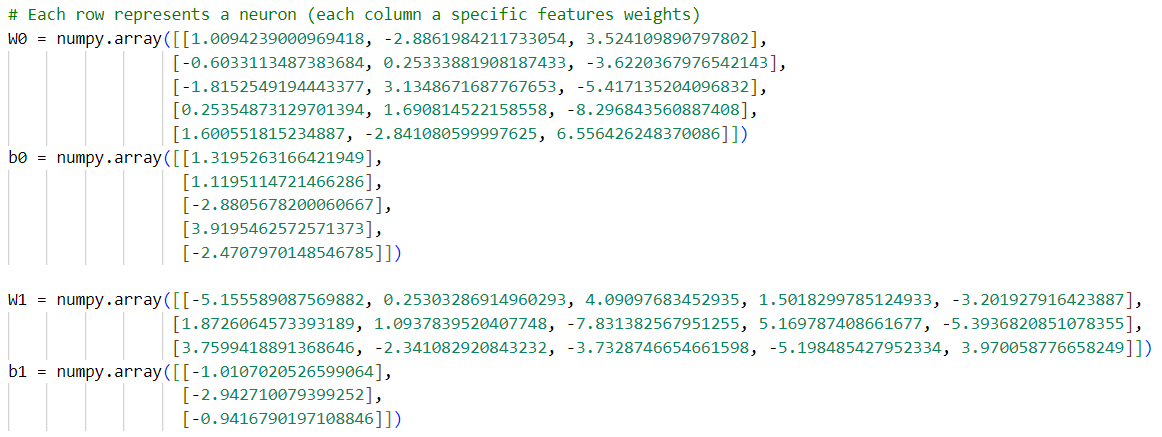
\includegraphics[width=1\textwidth]{parameters.png}
    \caption{Model Parameters}
    \label{fig:parameters}
\end{figure}

\begin{verbatim}
import numpy


def softmax(x):
    x_shifted = x - numpy.max(x, axis=1, keepdims=True)
    e_x = numpy.exp(x_shifted)
    return e_x / e_x.sum(axis=1, keepdims=True)


def sigmoid(X):
    return 1 / (1 + numpy.exp(-X))


# Each column represents a data point (each row a feature)
X = numpy.genfromtxt('iris-new-test.csv', delimiter=",")[:, :-1].T
min_vals = X.min(axis=0)
max_vals = X.max(axis=0)
X = (2 * X - min_vals - max_vals) / (max_vals - min_vals)

# Each row represents a neuron (each column a specific features weights)
W0 = numpy.array([[1.0094239000969418, -2.8861984211733054, 3.524109890797802],
                 [-0.6033113487383684, 0.25333881908187433, -3.6220367976542143],
                 [-1.8152549194443377, 3.1348671687767653, -5.417135204096832],
                 [0.25354873129701394, 1.690814522158558, -8.296843560887408],
                 [1.600551815234887, -2.841080599997625, 6.556426248370086]])
b0 = numpy.array([[1.3195263166421949], 
                  [1.1195114721466286], 
                  [-2.8805678200060667], 
                  [3.9195462572571373], 
                  [-2.4707970148546785]])

W1 = numpy.array([[-5.155589087569882, 0.25303286914960293, 4.09097683452935, 1.5018299785124933, -3.201927916423887],
                 [1.8726064573393189, 1.0937839520407748, -7.831382567951255, 5.169787408661677, -5.3936820851078355],
                 [3.7599418891368646, -2.341082920843232, -3.7328746654661598, -5.198485427952334, 3.970058776658249]])
b1 = numpy.array([[-1.0107020526599064], 
                  [-2.942710079399252], 
                  [-0.9416790197108846]])


print(X.shape)
print(W0.shape)
Y = softmax(W1 @ sigmoid(W0 @ X + b0) +b1)
print(Y)
Y = numpy.argmax(Y, axis=0).T
print(Y)
class_names = numpy.array(['Iris-setosa', 'Iris-versicolor', 'Iris-virginica'])
Y = class_names[Y]
print(Y)
\end{verbatim}


\begin{table}[H]
    \centering
    \caption{Final Results}
    \begin{tabular}{|c|ccc|ccc|c|}
        \hline
         & \multicolumn{3}{|c|}{Predicted In Python} & \multicolumn{3}{|c|}{Predicted In WEKA} & Actual \\
        \cline{2-7}
         & Iris-setosa & Iris-versicolor & Iris-virginica & Iris-setosa & Iris-versicolor & Iris-virginica & \\
        \hline
        1 & \textbf{0.9969} & 0.0031 & 0.0000 & \textbf{0.8276} & 0.1724 & 0.0000 & Iris-setosa \\
        \hline
        2 & 0.2236 & \textbf{0.7763} & 0.0001 & 0.3344 & \textbf{0.6575} & 0.0081 & Iris-setosa \\
        \hline
        3 & \textbf{0.9978} & 0.0022 & 0.0000 & \textbf{0.8265} & 0.1735 & 0.0000 & Iris-setosa \\
        \hline
        4 & \textbf{0.9940} & 0.0060 & 0.0000 & \textbf{0.8264} & 0.1736 & 0.0000 & Iris-setosa \\
        \hline
        5 & \textbf{0.9969} & 0.0031 & 0.0000 & \textbf{0.8283} & 0.1717 & 0.0000 & Iris-setosa \\
        \hline
        6 & \textbf{0.9572} & 0.0428 & 0.0000 & 0.8187 & \textbf{0.1813} & 0.0000 & Iris-setosa \\
        \hline
        7 & \textbf{0.9983} & 0.0017 & 0.0000 & \textbf{0.8284} & 0.1716 & 0.0000 & Iris-setosa \\
        \hline
        8 & \textbf{0.9944} & 0.0056 & 0.0000 & \textbf{0.8262} & 0.1738 & 0.0000 & Iris-setosa \\
        \hline
        9 & \textbf{0.9959} & 0.0041 & 0.0000 & \textbf{0.8282} & 0.1718 & 0.0000 & Iris-setosa \\
        \hline
        10 & \textbf{0.9886} & 0.0114 & 0.0000 & \textbf{0.8267} & 0.1733 & 0.0000 & Iris-setosa \\
        \hline
        11 & 0.0000 & 0.0046 & \textbf{0.9954} & 0.0595 & \textbf{0.7754} & 0.1651 & Iris-versicolor \\
        \hline
        12 & 0.0003 & 0.2487 & \textbf{0.7510} & 0.0656 & \textbf{0.7854} & 0.1490 & Iris-versicolor \\
        \hline
        13 & 0.0004 & \textbf{0.7998} & 0.1998 & 0.0527 & \textbf{0.7613} & 0.1859 & Iris-versicolor \\
        \hline
        14 & 0.0003 & \textbf{0.9762} & 0.0235 & 0.0597 & \textbf{0.7757} & 0.1646 & Iris-versicolor \\
        \hline
        15 & 0.0003 & 0.2420 & \textbf{0.7578} & 0.0508 & \textbf{0.7566} & 0.1926 & Iris-versicolor \\
        \hline
        16 & 0.0004 & \textbf{0.7612} & 0.2384 & \textbf{0.2807} & 0.7062 & 0.0130 & Iris-versicolor \\
        \hline
        17 & 0.0004 & \textbf{0.6290} & 0.3705 & 0.1026 & \textbf{0.8115} & 0.0859 & Iris-versicolor \\
        \hline
        18 & 0.0004 & \textbf{0.8611} & 0.1385 & 0.0727 & \textbf{0.7944} & 0.1329 & Iris-versicolor \\
        \hline
        19 & 0.0001 & \textbf{0.9997} & 0.0002 & 0.0725 & \textbf{0.7942} & 0.1334 & Iris-versicolor \\
        \hline
        20 & 0.0004 & \textbf{0.7380} & 0.2615 & 0.0672 & \textbf{0.7876} & 0.1452 & Iris-versicolor \\
        \hline
        21 & 0.0000 & 0.0001 & \textbf{0.9999} & 0.0015 & 0.3527 & \textbf{0.6458} & Iris-virginica \\
        \hline
        22 & 0.0002 & 0.1910 & \textbf{0.8088} & 0.0015 & 0.3529 & \textbf{0.6456} & Iris-virginica \\
        \hline
        23 & 0.0000 & 0.0000 & \textbf{0.9999} & 0.0021 & 0.3620 & \textbf{0.6359} & Iris-virginica \\
        \hline
        24 & 0.0000 & 0.0000 & \textbf{0.9999} & 0.0015 & 0.3530 & \textbf{0.6455} & Iris-virginica \\
        \hline
        25 & 0.0000 & 0.0001 & \textbf{0.9999} & 0.0015 & 0.3526 & \textbf{0.6459} & Iris-virginica \\
        \hline
        26 & 0.0000 & 0.0159 & \textbf{0.9841} & 0.0015 & 0.3529 & \textbf{0.6456} & Iris-virginica \\
        \hline
        27 & 0.0000 & 0.0007 & \textbf{0.9993} & 0.0019 & 0.3599 & \textbf{0.6382} & Iris-virginica \\
        \hline
        28 & 0.0000 & 0.0031 & \textbf{0.9969} & 0.0017 & 0.3566 & \textbf{0.6417} & Iris-virginica \\
        \hline
        29 & 0.0000 & 0.0001 & \textbf{0.9999} & 0.0016 & 0.3534 & \textbf{0.6451} & Iris-virginica \\
        \hline
        30 & 0.0000 & 0.0000 & \textbf{0.9999} & 0.0032 & 0.3843 & \textbf{0.6125} & Iris-virginica \\
        \hline
    \end{tabular}
\end{table}

In the table above python predictions don't match the WEKA predictions because I removed the wrong column in WEKA (index 3 - which is the 4th column).  Theoretically predicted probabilities should match fully, because it doesn't matter in what environment the calculations are executed.

    
\end{document}